%====================================================================================================
\chapter{Development of a Simple Emulator for L0 Muon Trigger System} \label{ch:L0MuonEmulator}
%====================================================================================================
This chapter introduces the development of a simple emulator, emulating the L0 muon trigger behavior on both barrel and endcap region, called L0MuonEmulator. The L0Muon-Emulator is a C++ based software package on Athena that emulates the trigger decision for muons as provided by the L0 trigger system for HL-LHC. The L0MuonEmulator makes decisions of whether a muon candidate should be accepted or rejected based on a pre-set step function of transverse momentum $p_\mathrm{T}$, and then outputs smeared $p_\mathrm{T}$ as the transverse momentum information in ROI (Region Of Interest). In this chapter, an overview of the emulator's design and logic is provided. Since the simulation based solely on smearing was insufficient to replicate the actual trigger logic, a masking procedure to make the trigger performance is also introduced to reproduce the angular acceptance of the L0 muon trigger system. The result of the emulation is presented along with a discussion about the need for a more precise simulation approach.
%====================================================================================================
\section{Purpose and Function of the Simple Emulator} \label{sec:L0MuonPurpose}
%====================================================================================================
The purpose of the L0MuonEmulator is to provide a temporary input interface for downstream development, the Event Filter (EF), which we introduced in Chapter~\ref{ch:ATLAS}. This emulator provides $p_\mathrm{T}$ and the ROI information of muons for further selection by EF. At present, the emulator takes the truth values of the four-momentum for all generated particles in a simulated event as an input. 

In practice, only final state muons and its anti-particles are used. These selected muons and anti-particles are then passed through a smearing and filtering procedure that models the detector resolution and trigger efficiency, providing a collection of RoI information based on the emulated L0 muon trigger. Each RoI contains information on transverse momentum ($p_\mathrm{T}$), pseudorapidity ($\eta$), azimuthal angle ($\phi$), and charge.

The filtering function in the L0MuonEmulator simulates the trigger efficiency as a function of muon transverse momentum. A simplified step-function model is implemented, in which muons below a certain threshold are discarded, while muons above that threshold are accepted with an efficiency of 95\%. This 95\% efficiency is approximately determined based on the efficiency of endcap in L1 muon trigger in Run~3 and the efficiency of barrel simulated for Phase-II upgrade, as shown in Section~\ref{sec:L0MuonEmulatorPerformance}. In addition, the emulator includes a basic geometric masking procedure to exclude regions outside the muon detector acceptance. Currently, this is implemented by discarding all truth muons with pseudorapidity $|\eta| > 2.41$, which roughly corresponds to the coverage limit of the L0 muon trigger chambers in ATLAS. Truth muons outside this region are automatically rejected.

The smearing algorithm emulates the detector resolution by applying a smearing function to the inverse transverse momentum ($q/p_\mathrm{T}$) of the selected muons. Currently, a Gaussian distribution is used as the smearing function, tentatively with a width of 5\% of the input $q/p_\mathrm{T}$. The $\eta$ and $\phi$ positions are not smeared at this stage, as the RoI granularity is coarser than the smearing scale, which thereby dominates the uncertainty. Once smeared, the kinematic variables are encoded into a bit-wise RoI word format compatible with the hardware-level representation used in the ATLAS trigger system.

In addition, the L0MuonEmulator provides a monitoring function based on the Athena Monitoring Framework. A series of histograms are produced during the execution to validate the emulator output with the input truth muon properties. These include distributions of $\eta$, $\phi$, $p_\mathrm{T}$, and $q/p_\mathrm{T}$ before and after smearing, as well as resolution plots such as $\Delta\eta$, $\Delta\phi$, and relative $p_\mathrm{T}$ deviation.

%====================================================================================================
\section{Muon Trigger Acceptance after Phase-II Upgrade} \label{sec:MuonTriggerAcceptance}
%====================================================================================================
As discussed in Chapter~\ref{ch:ATLAS}, at the barrel region of the ATLAS detector, there are some dead zones in the RPC detector, affecting the trigger acceptance and efficiency. Therefore, a new station of RPC detector in the BI region will be added in Phase-II upgrade. This additional RPC0 enables a four-layer RPC configuration and allows for more flexible coincidence schemes. A summary of the logic combinations is provided in Table~\ref{tab:RPC_coincidence_modes}. Three coincidence schemes are considered ``3/3 chambers'', ``3/4 chambers'', and ``3/4 chambers + BI-BO'', which are defined by the number of required stations to register hits of the barrel detector. 

The performance of muon trigger acceptance in the barrel region for ``3/3 chambers'' in Run~3  are shown in Figure~\ref{fig:trigger_acceptance_3_3}. Figure~\ref{fig:trigger_acceptance_3_4} and Figure~\ref{fig:trigger_acceptance_3_4_BI_BO} shows the acceptance for ``3/4 chambers'', and ``3/4 chambers + BI-BO'' schemes in Run~4, respectively. From these pictures, we can see that the trigger acceptance gradually improves through the Phase-II upgrade, with the highest coverage achieved in the ``3/4 chambers + BI-BO'' pattern.

\begin{table}[htbp]
  \centering
  \caption{Hit requirements for different RPC trigger coincidence modes.}
  \label{tab:RPC_coincidence_modes}
  \begin{tabular}{lccc}
    \hline
    Requirement & RPC0 (BI) & BM (RPC1+2) & RPC3 (BO) \\
    \hline
    3/3 chambers          & --         & 3 out of 4 & 1 out of 2 \\
    \hline
    3/4 chambers          & --         & 3 out of 4 & 1 out of 2 \\
                          & 2 out of 3 & \multicolumn{2}{c}{3 out of 6} \\
    \hline
    3/4 chambers + BI-BO  & --         & 3 out of 4 & 1 out of 2 \\
                          & 2 out of 3 & \multicolumn{2}{c}{3 out of 6} \\
                          & 2 out of 3 & --         & 1 out of 2 \\
    \hline
  \end{tabular}
\end{table}

\begin{figure}[htbp]
  \centering
  \begin{subfigure}{0.67\textwidth}
    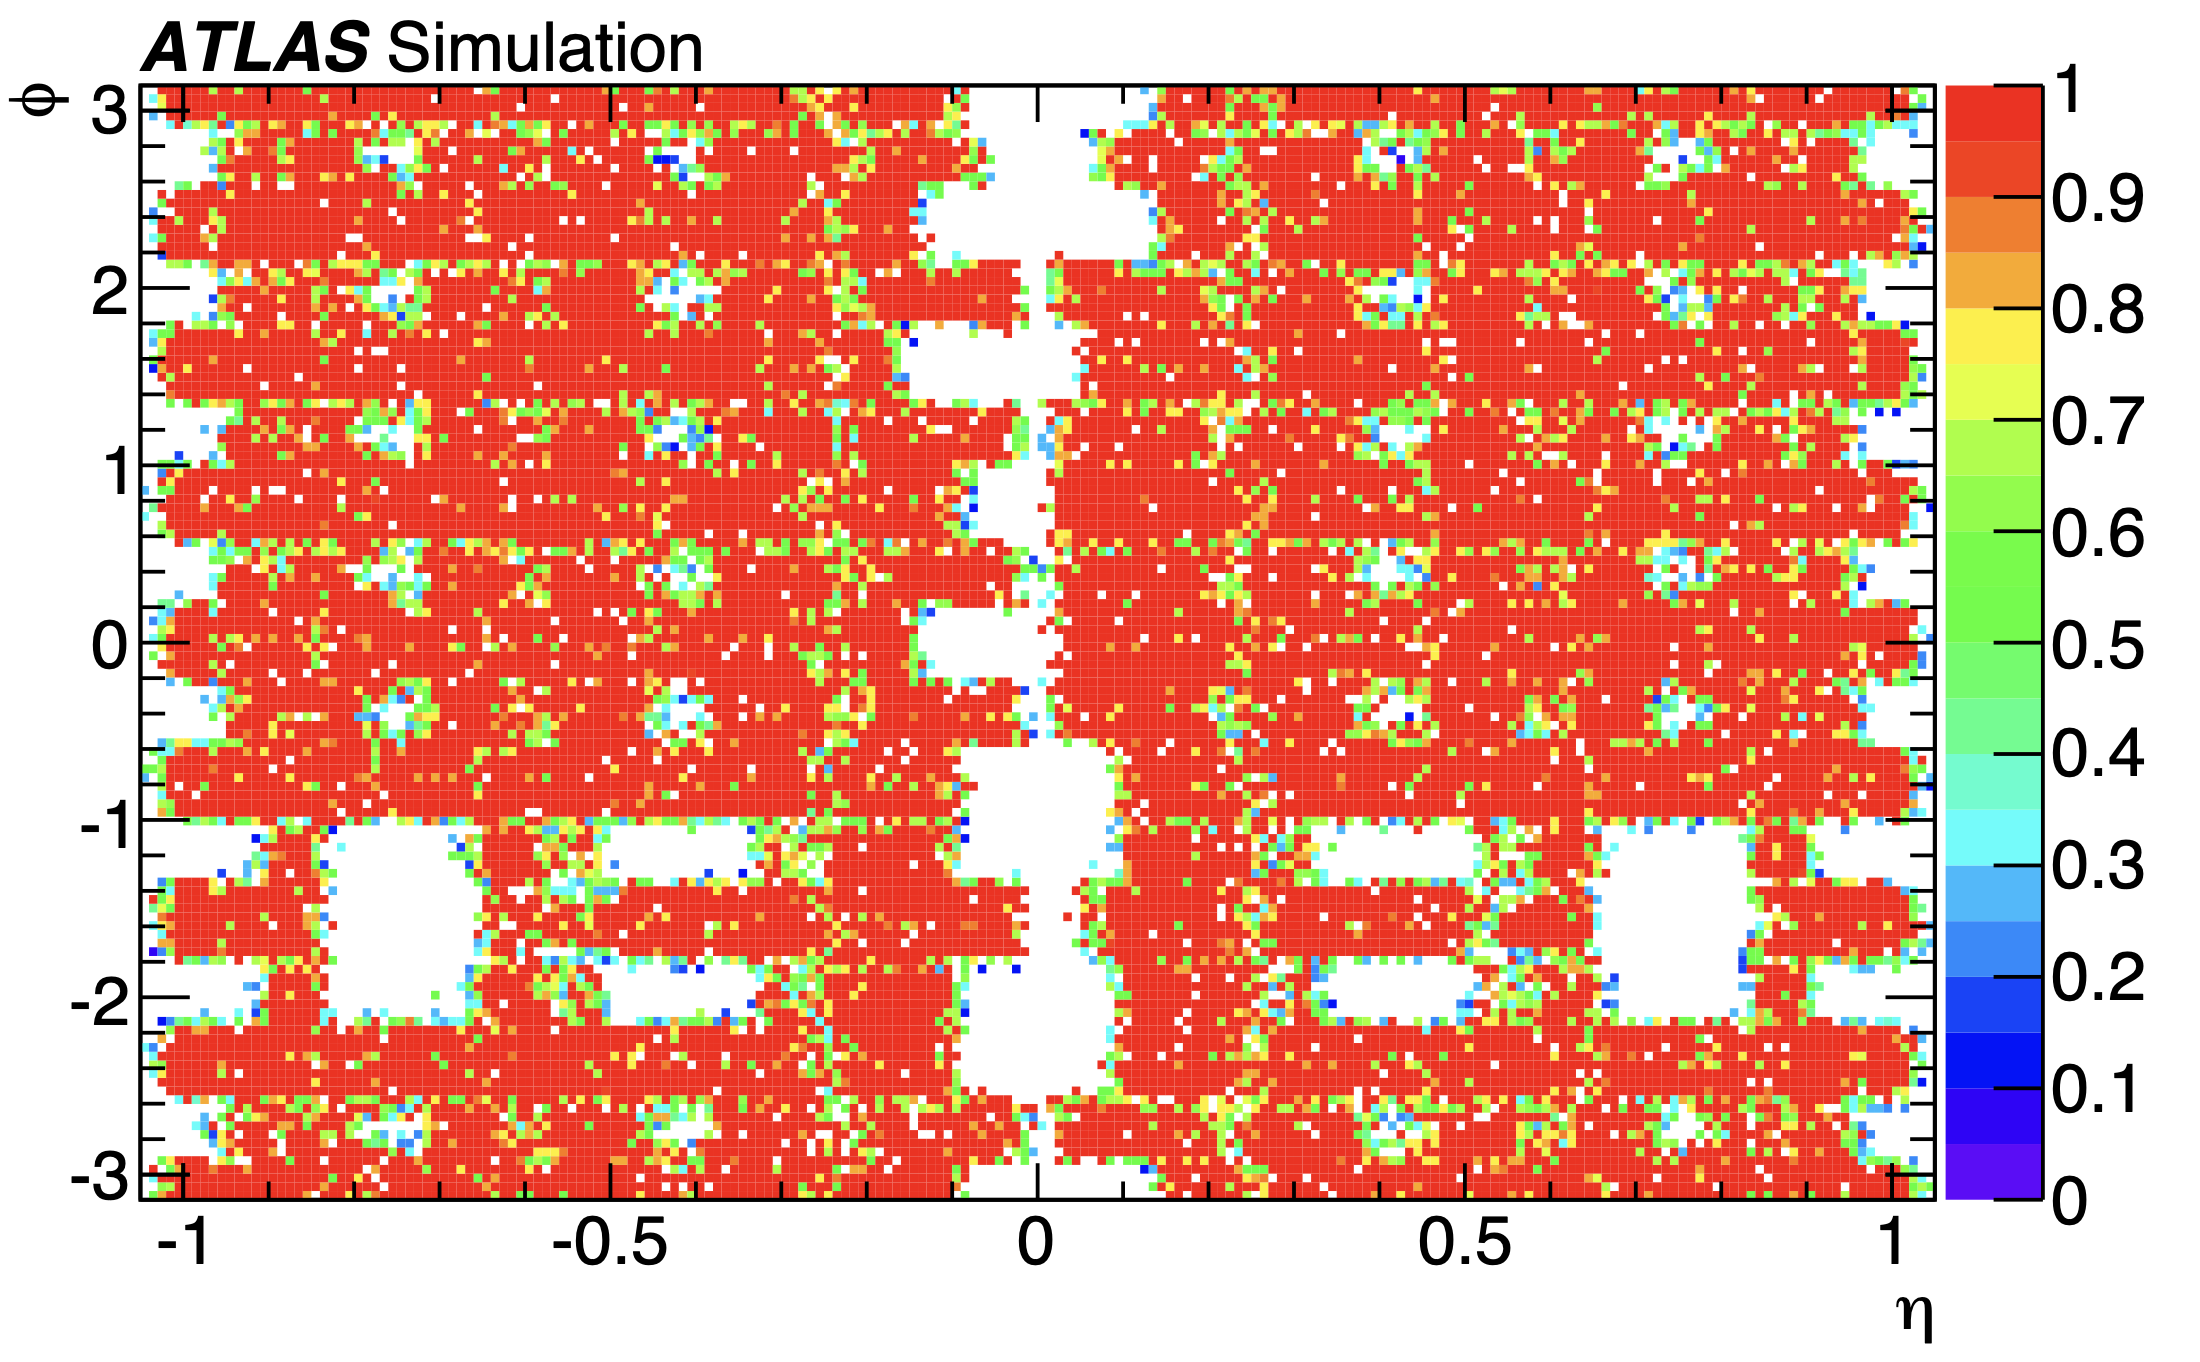
\includegraphics[width=\textwidth]{figs/chapter4/trigger_acceptance_map_3_3.png}
    \caption{3/3 chambers}
    \label{fig:trigger_acceptance_3_3}
  \end{subfigure}

  % \vspace{0.1cm} % 图之间的竖直间距

  \begin{subfigure}{0.67\textwidth}
    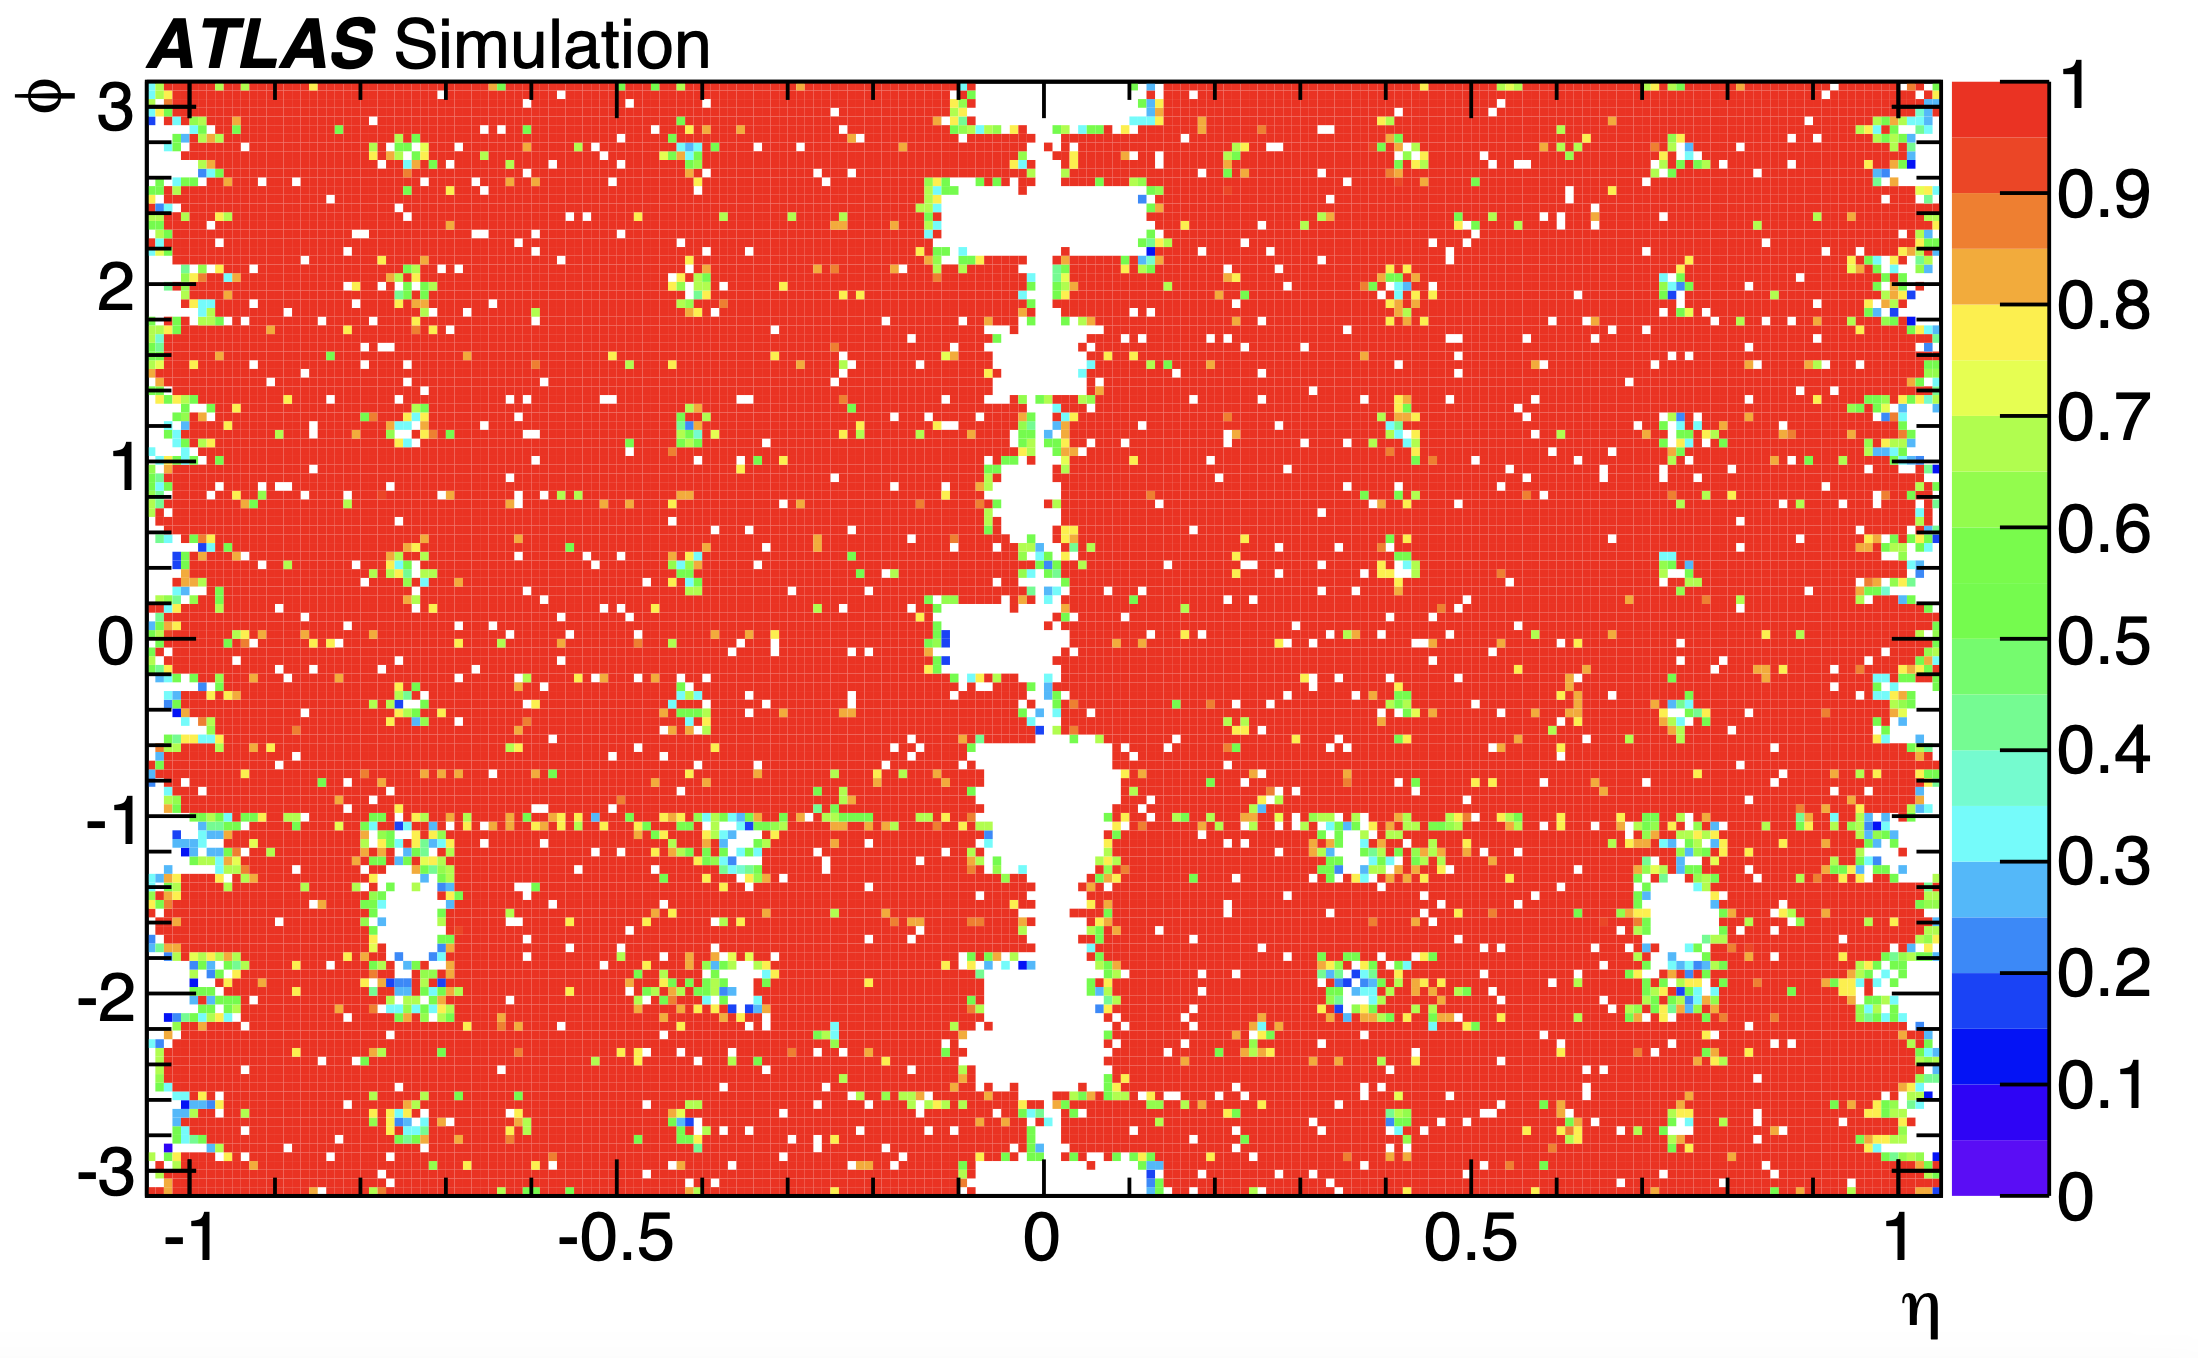
\includegraphics[width=\textwidth]{figs/chapter4/trigger_acceptance_map_3_4.png}
    \caption{3/4 chambers}
    \label{fig:trigger_acceptance_3_4}
  \end{subfigure}

  % \vspace{0.1cm}

  \begin{subfigure}{0.67\textwidth}
    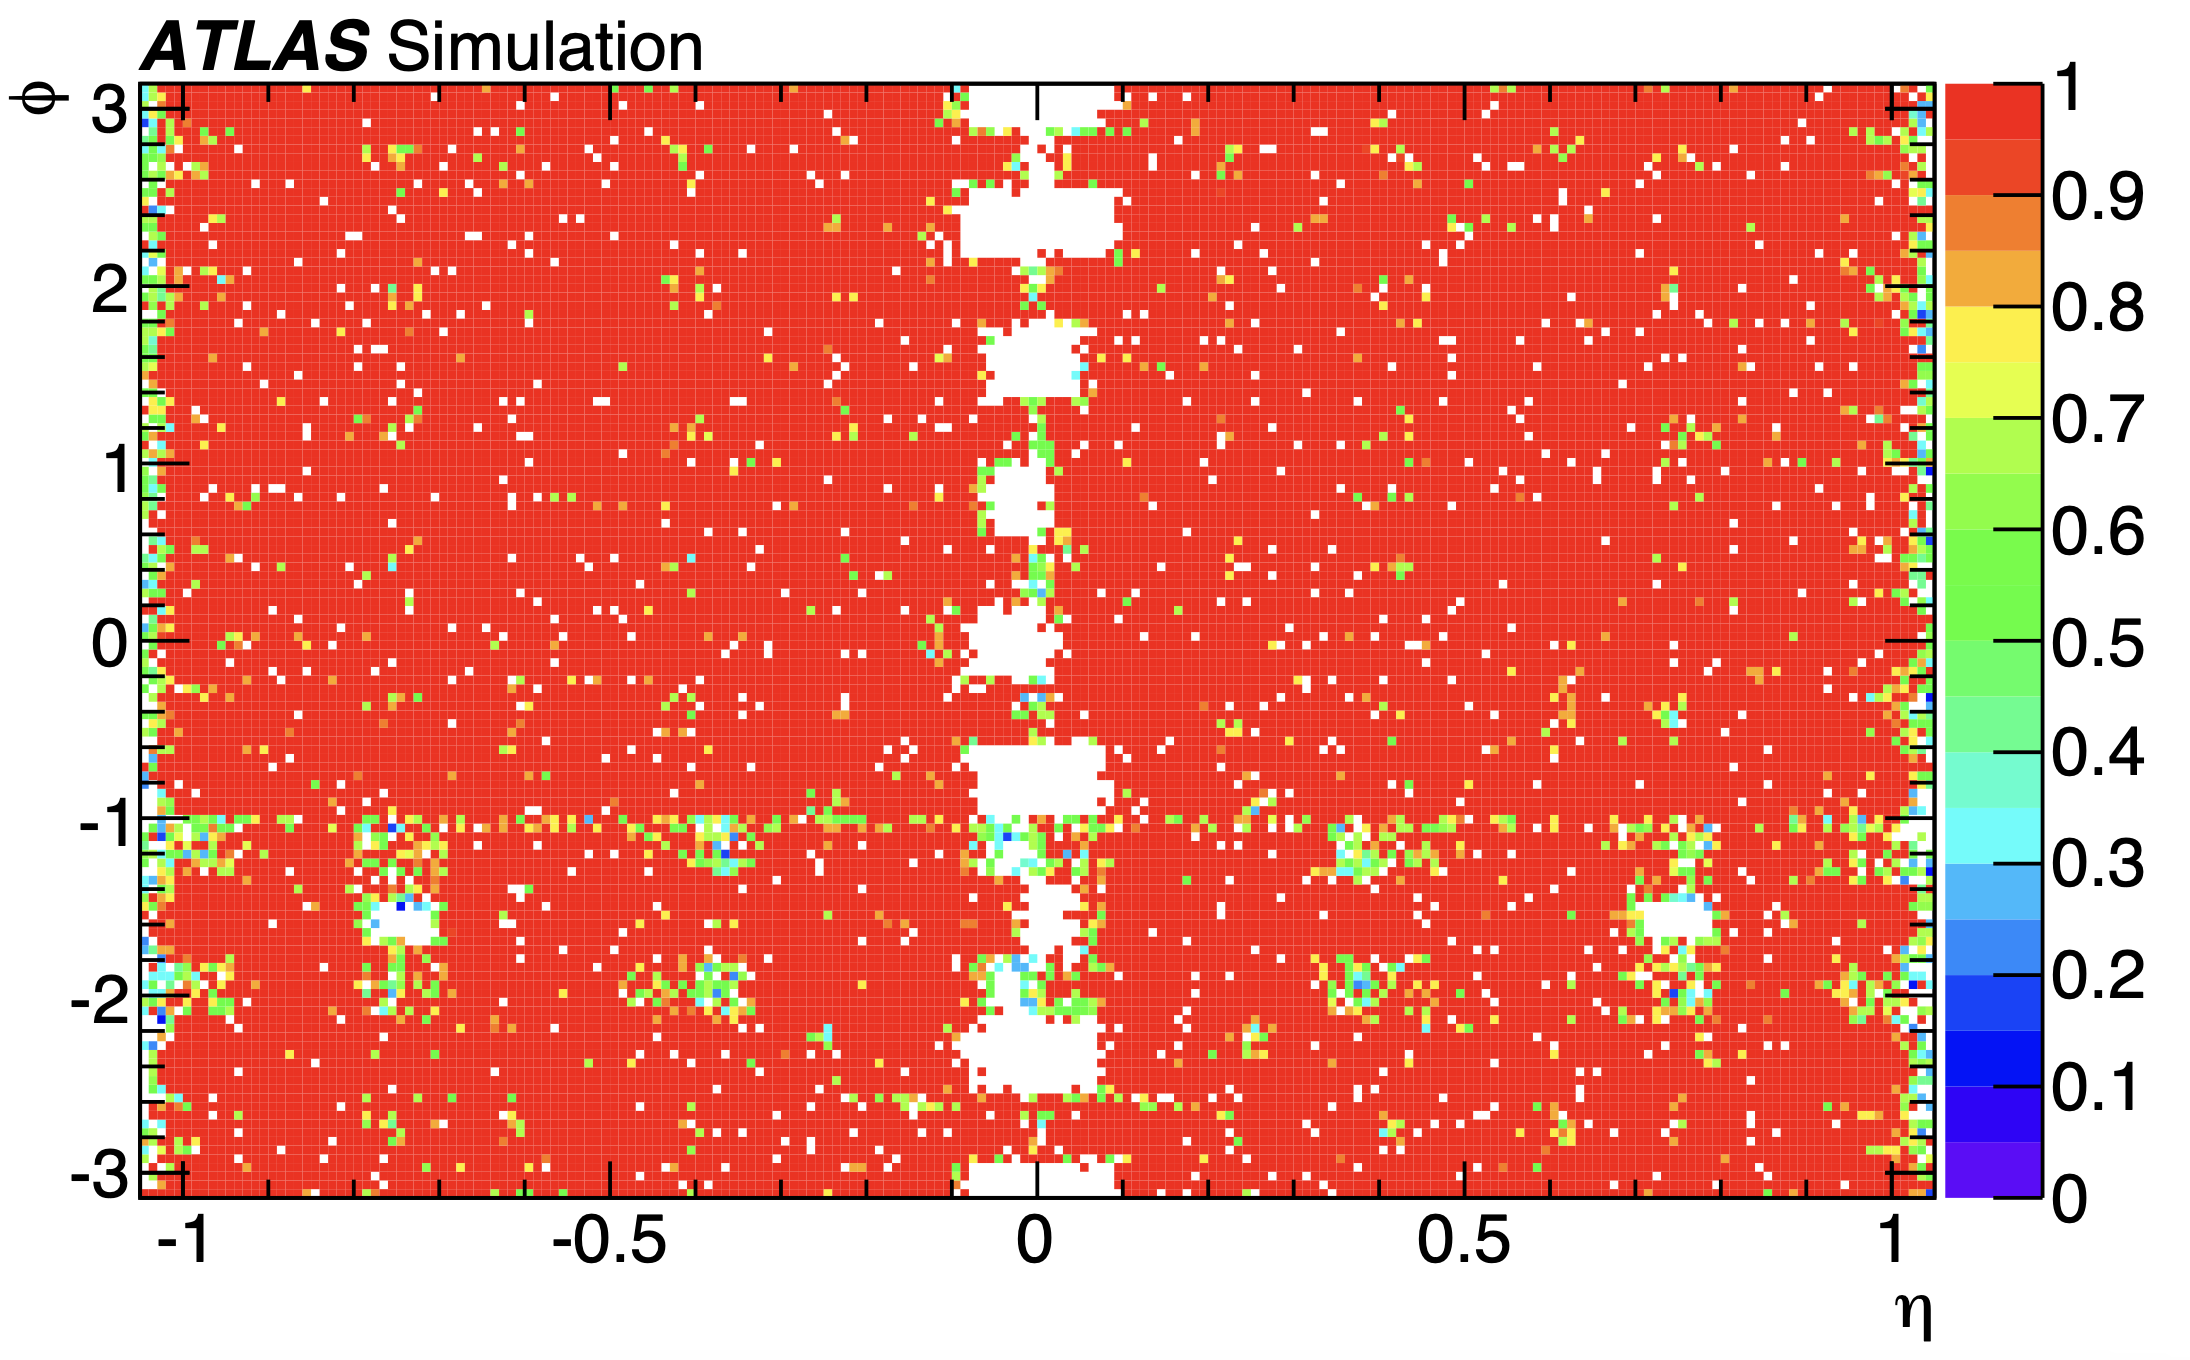
\includegraphics[width=\textwidth]{figs/chapter4/trigger_acceptance_map_3_4_BI_BO.png}
    \caption{3/4 chambers + BI-BO}
    \label{fig:trigger_acceptance_3_4_BI_BO}
  \end{subfigure}

  \caption{Trigger acceptance maps in $\eta$-$\phi$ space for different coincidence logics \cite{TDAQ_TDR}.}
  \label{fig:trigger_acceptance_all}
\end{figure}
%====================================================================================================
\section{Simulation for the trigger acceptance} 
%====================================================================================================
Section~\ref{sec:MuonTriggerAcceptance} above shows that even applying the coincidence scheme with highest acceptance, some unavoidable holes remain due to mechanical limitations. In this section, a simple simulation that emulates the barrel muon trigger acceptance in Run~4 are implemented. This emulates the ``holes'' caused by mechanical structures based on the ``3/4 chambers + BI-BO'' scheme, which shows the highest coverage.

As described in Section~\ref{sec:L0MuonPurpose}, the original implementation adopted a simplified geometric acceptance cut by discarding all truth muons with pseudorapidity $|\eta| > 2.41$, roughly corresponding to the nominal detector coverage of the L0 muon chambers. To further filter those ``holes'', specific $(\eta, \phi)$ masking scheme corresponding to uncovered regions are manually excluded within the smearing algorithm. Figure~\ref{fig:masking} shows those excluded regions, which are enclosed by blue dashed lines.

\begin{figure}[htbp]
  \centering
  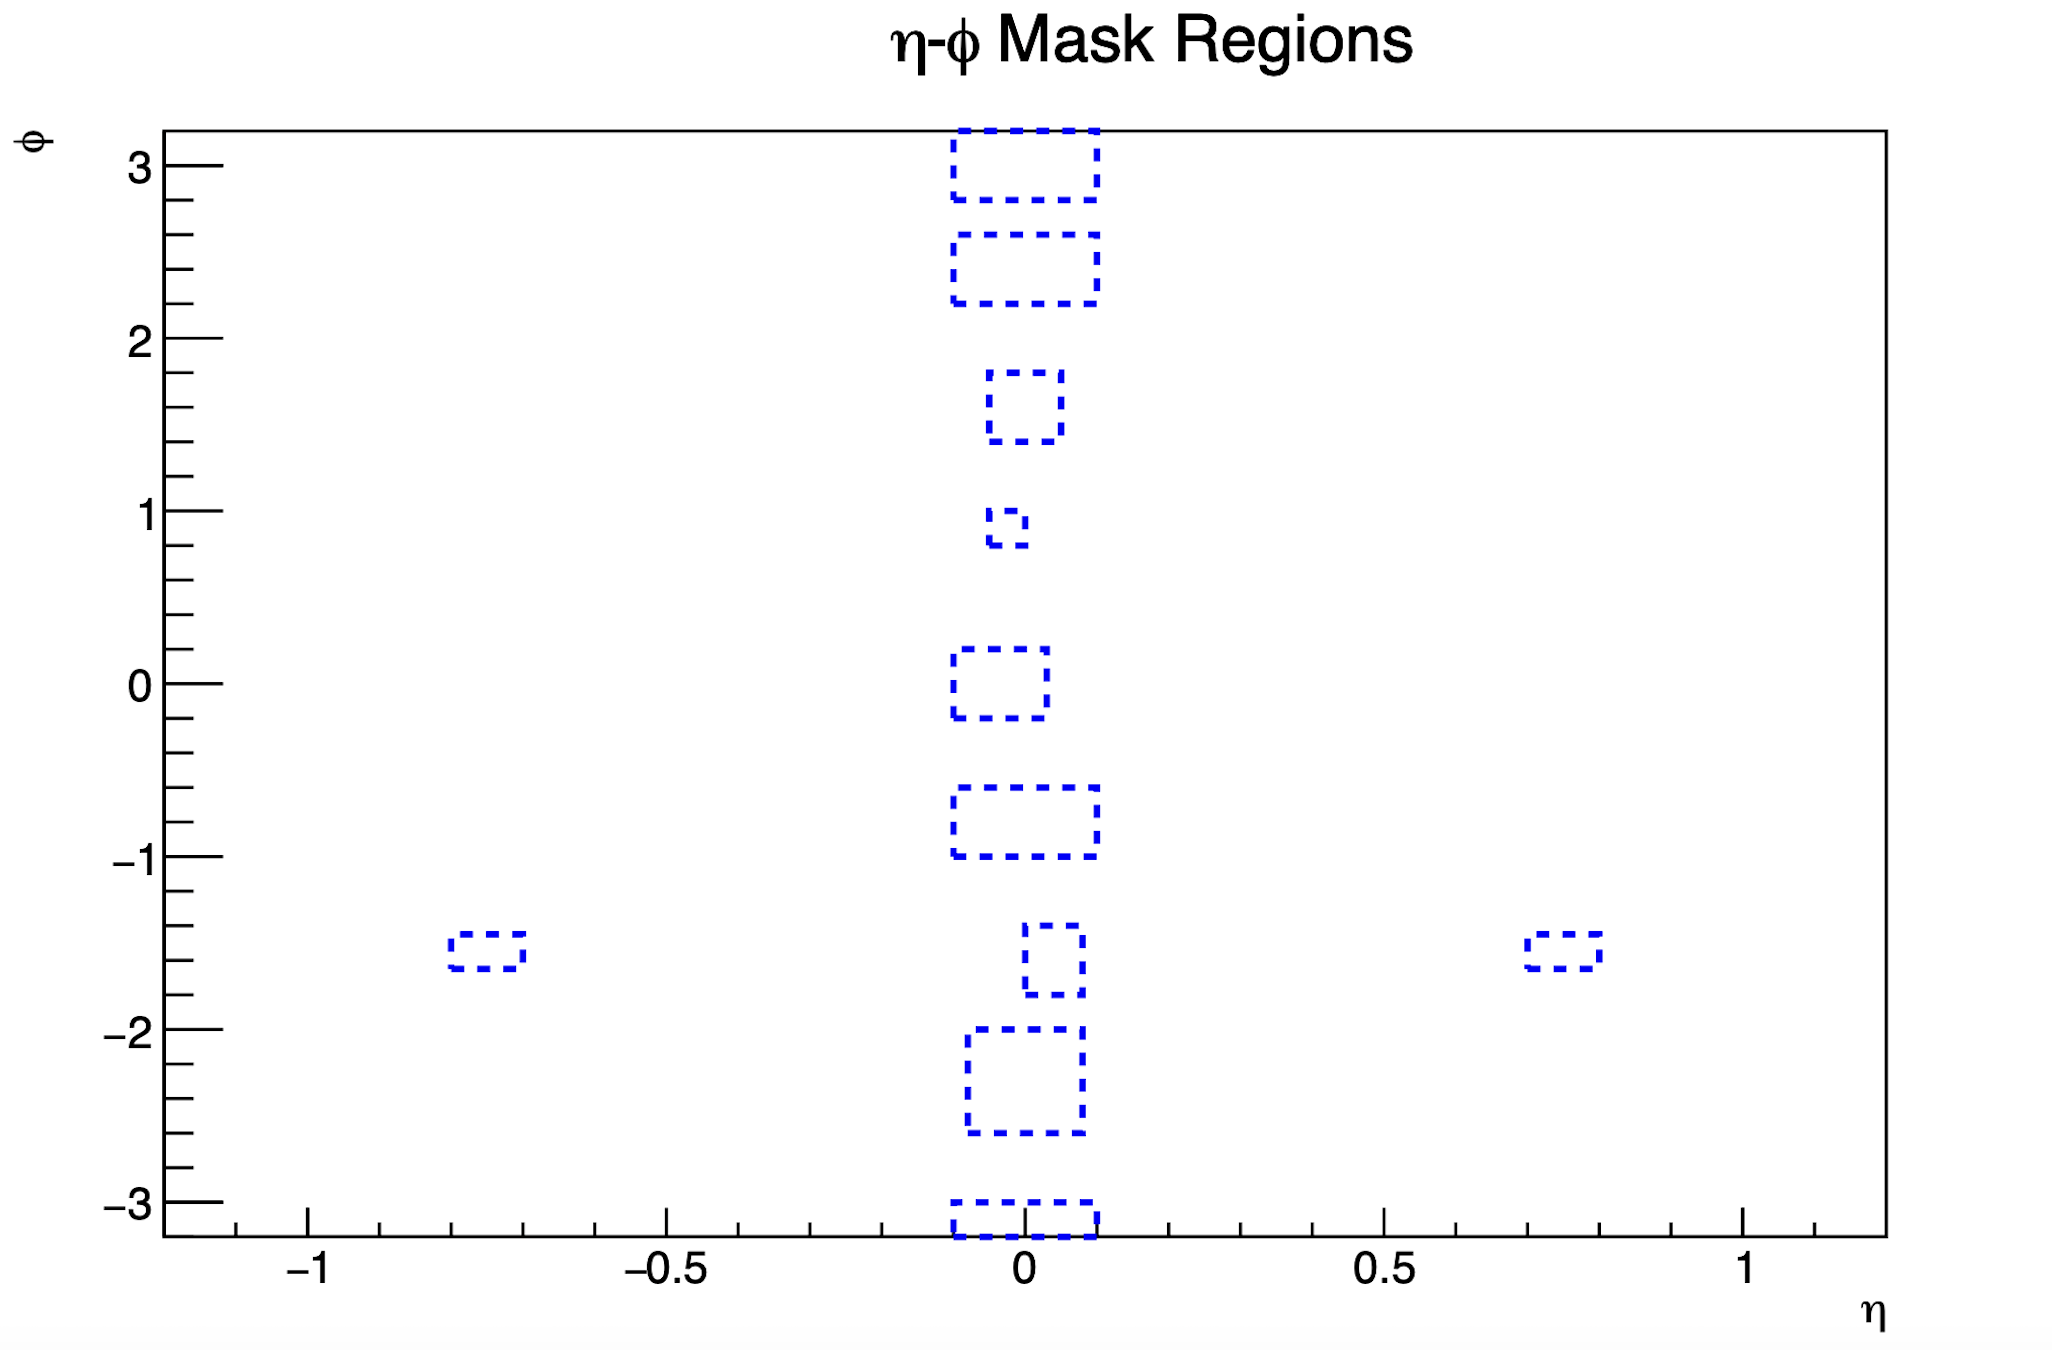
\includegraphics[width=0.85\textwidth]{figs/chapter4/masked_eta_phi_map.png}
  \caption{Masked region for simulation of barrel muon trigger acceptance.}
  \label{fig:masking}
\end{figure}

%====================================================================================================
\section{Performance of the L0MuonEmulator} \label{sec:L0MuonEmulatorPerformance}
%====================================================================================================
In this section, the efficiency of the L0MuonEmulator is compared to the references of the trigger efficiency in Run~3 for endcap, and Run~4 for barrel with higher efficiency being performed. The data file used for the efficiency calculation is a Monte Carlo sample of $Z \to \mu^+ \mu^-$ events at a center-of-mass energy of $13.6\,\mathrm{TeV}$, with a total of $60{,}000$ events.

Figure~\ref{fig:L1MuonEndcapEff} shows the muon trigger efficiencies in the endcap region with several $p_\mathrm{T}$ thresholds, using experimental data from LHC Run~3. Figure~\ref{fig:L0MuonBarrelEff} gives the barrel muon trigger efficiencies with four steps of $p_\mathrm{T}$ thresholds based on simulation for Phase-II upgrade. Figure~\ref{fig:eff_pt_endcap} and Figure~\ref{fig:eff_pt_barrel} show the efficiencies of the L0MuonEmulator in endcap and barrel regions with five thresholds, respectively. The efficiency is defined in Equation~\ref{eq:emulator_efficiency}. 

\begin{equation}
\label{eq:emulator_efficiency}
\mathrm{Efficiency} = \frac{\text{Muons selected by the filtering function}}{\text{All the truth muons}}
\end{equation}

As a result, the turn-on curves are reproduced by the L0MuonEmulator, showing a fair agreement with the references.

% --------- 第一页 两张图 ---------
\begin{figure}[htbp]
  \centering
  \hspace{-1cm}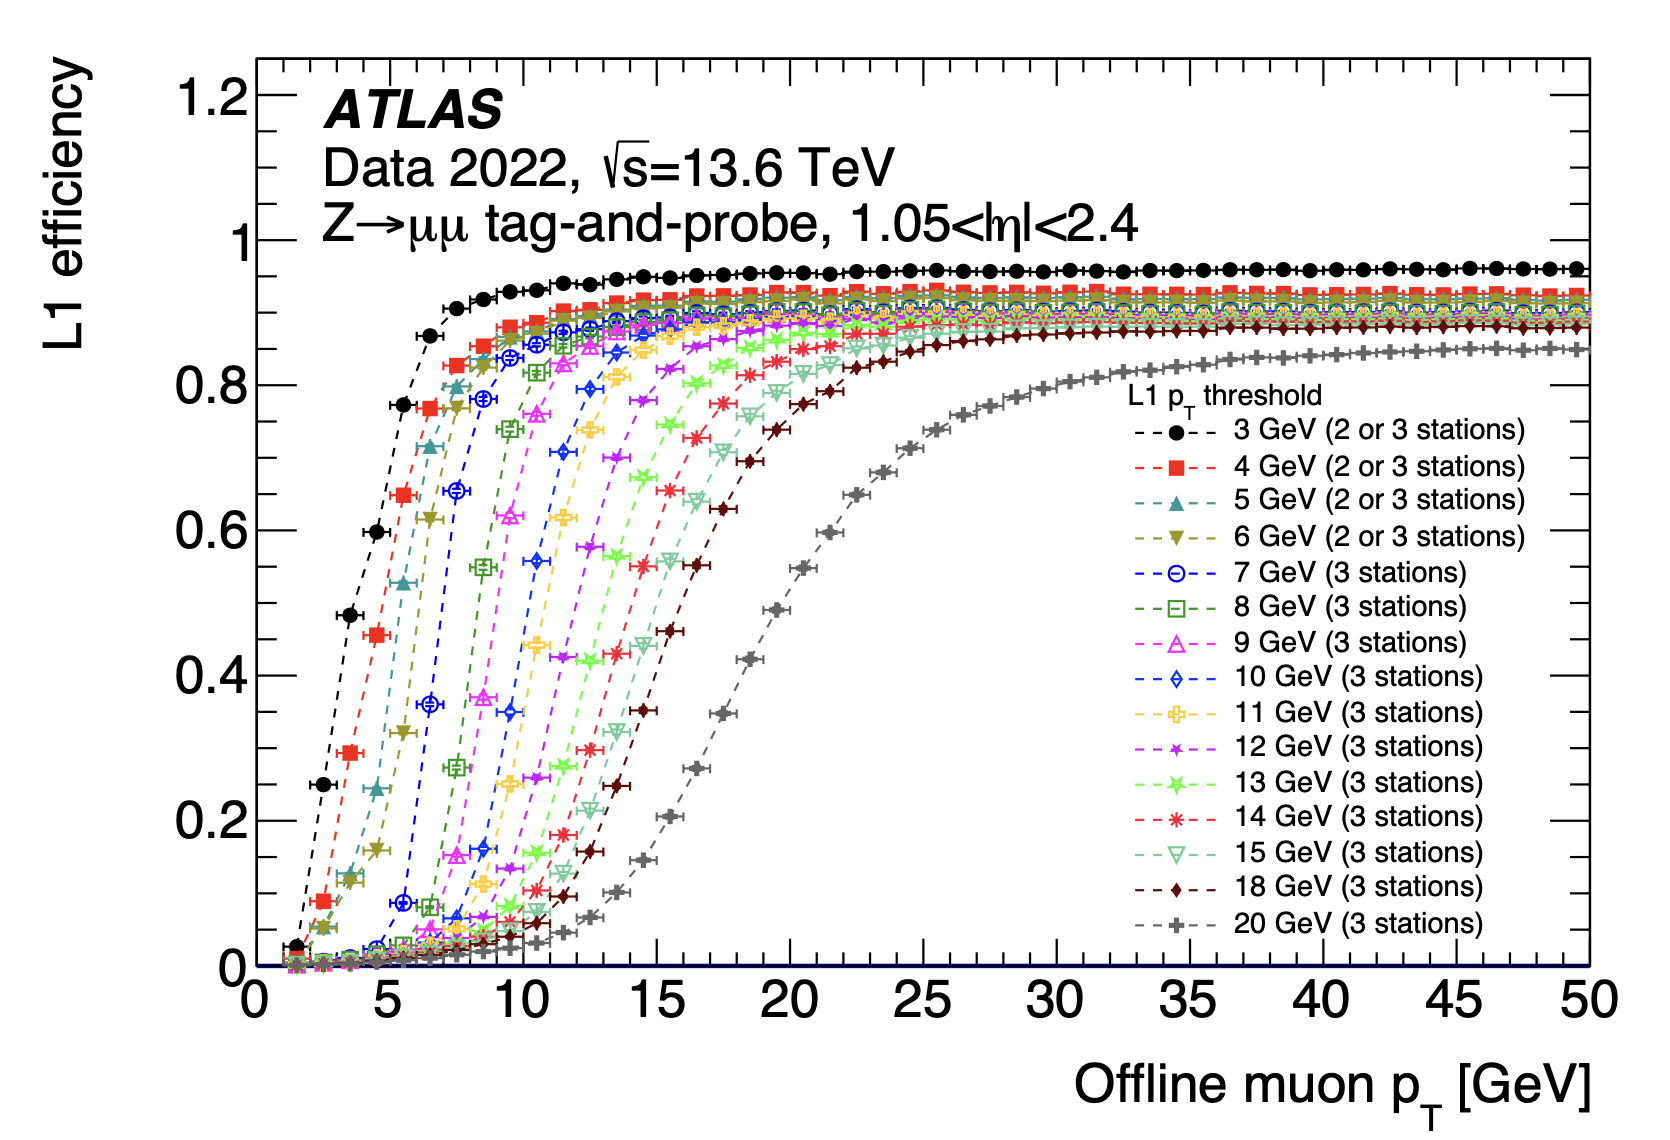
\includegraphics[width=0.90\textwidth]{figs/chapter4/L1Muon_endcap_eff.png}
  \caption{Efficiency of L1 muon triggers in the endcap region for several $p_\mathrm{T}$ thresholds \cite{ATLASRun3Trigger}.}
  \label{fig:L1MuonEndcapEff}

  % \vspace{0.2cm} % 图之间的竖直间距

  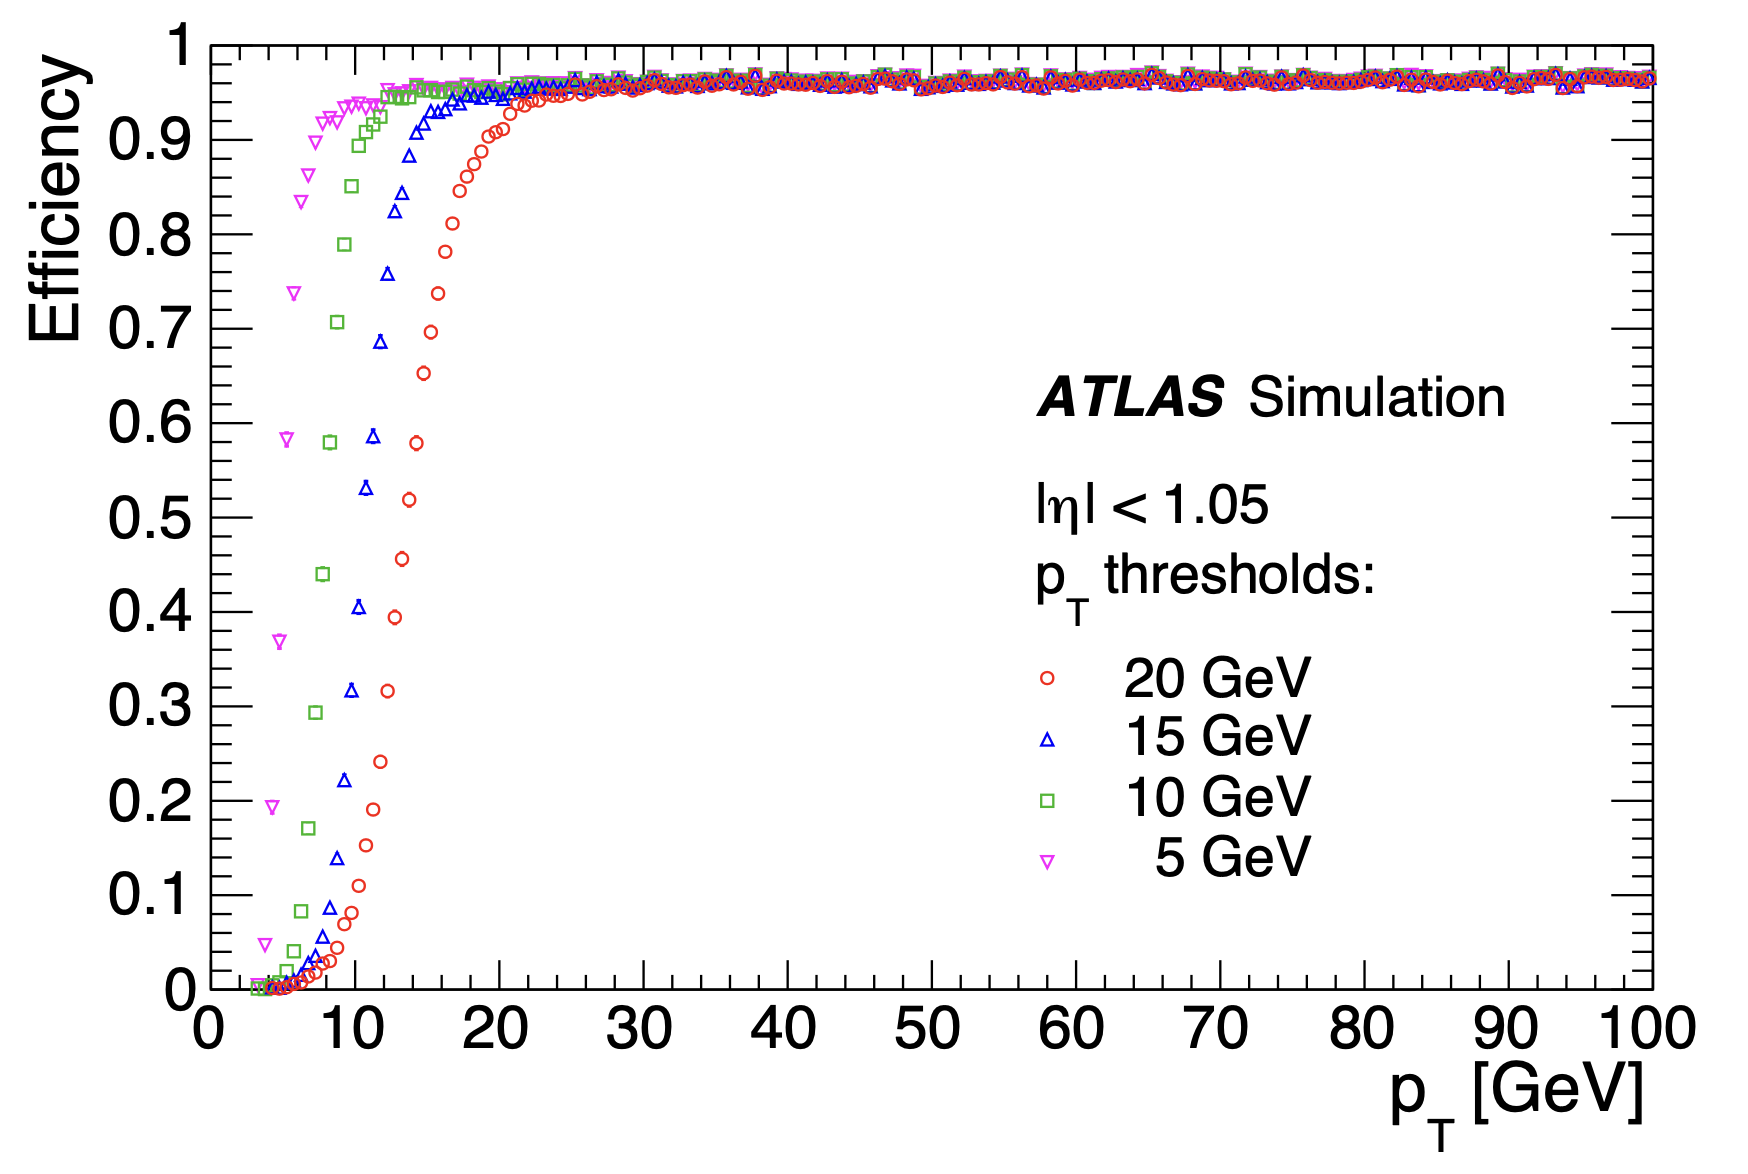
\includegraphics[width=0.88\textwidth]{figs/chapter4/L0Muon_barrel_eff.png}
  \caption{Efficiency of RPC L0 muon triggers in the barrel region for different $p_\mathrm{T}$ thresholds using ``3/4 chambers + BI-BO'' scheme \cite{TDAQ_TDR}.}
  \label{fig:L0MuonBarrelEff}
\end{figure}

% --------- 第二页 两张图 ---------
\begin{figure}[htbp]
  \centering
  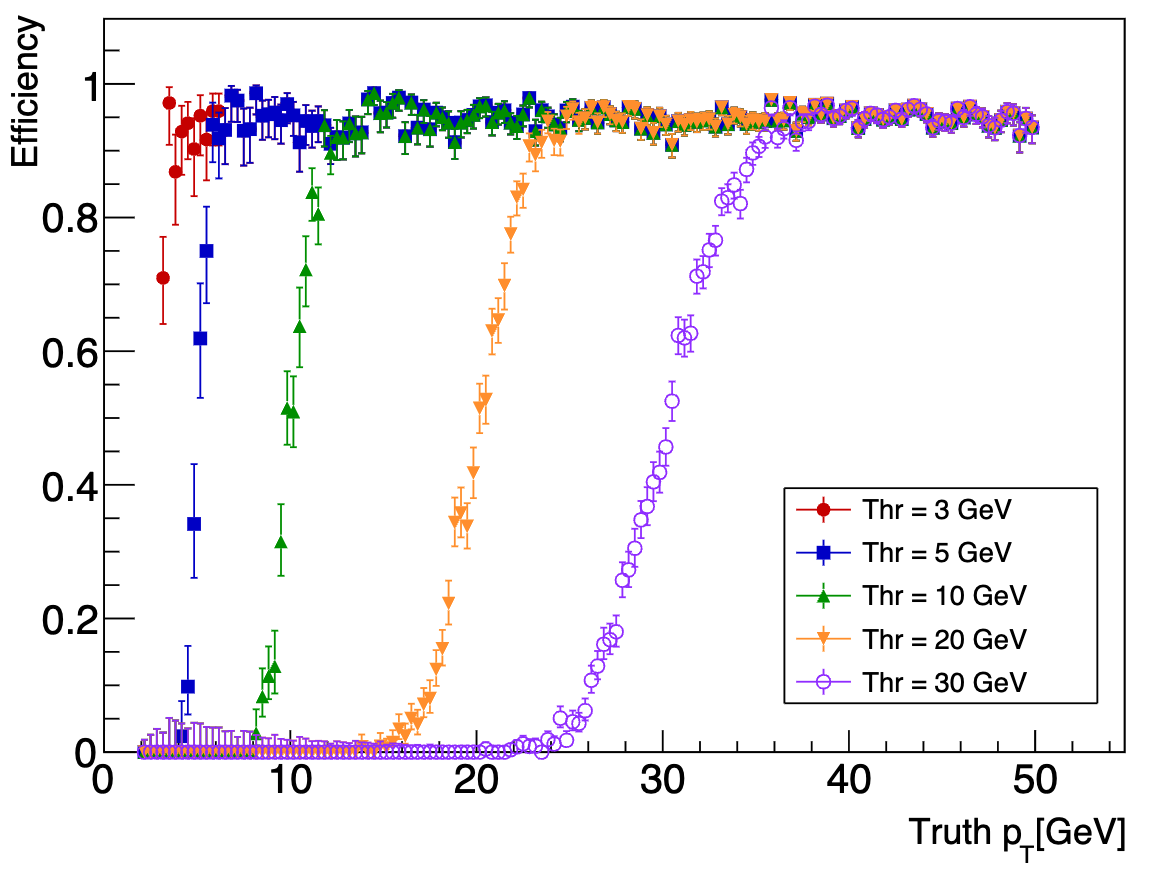
\includegraphics[width=0.83\textwidth]{figs/chapter4/efficiency_endcap_multi_right_new_new.png}
  \caption{Efficiency of L0MuonEmulator in the endcap region for five $p_\mathrm{T}$ thresholds: 3~GeV, 5~GeV, 10~GeV, 20~GeV, 30~GeV.}
  \label{fig:eff_pt_endcap}

  % \vspace{0.2cm}

  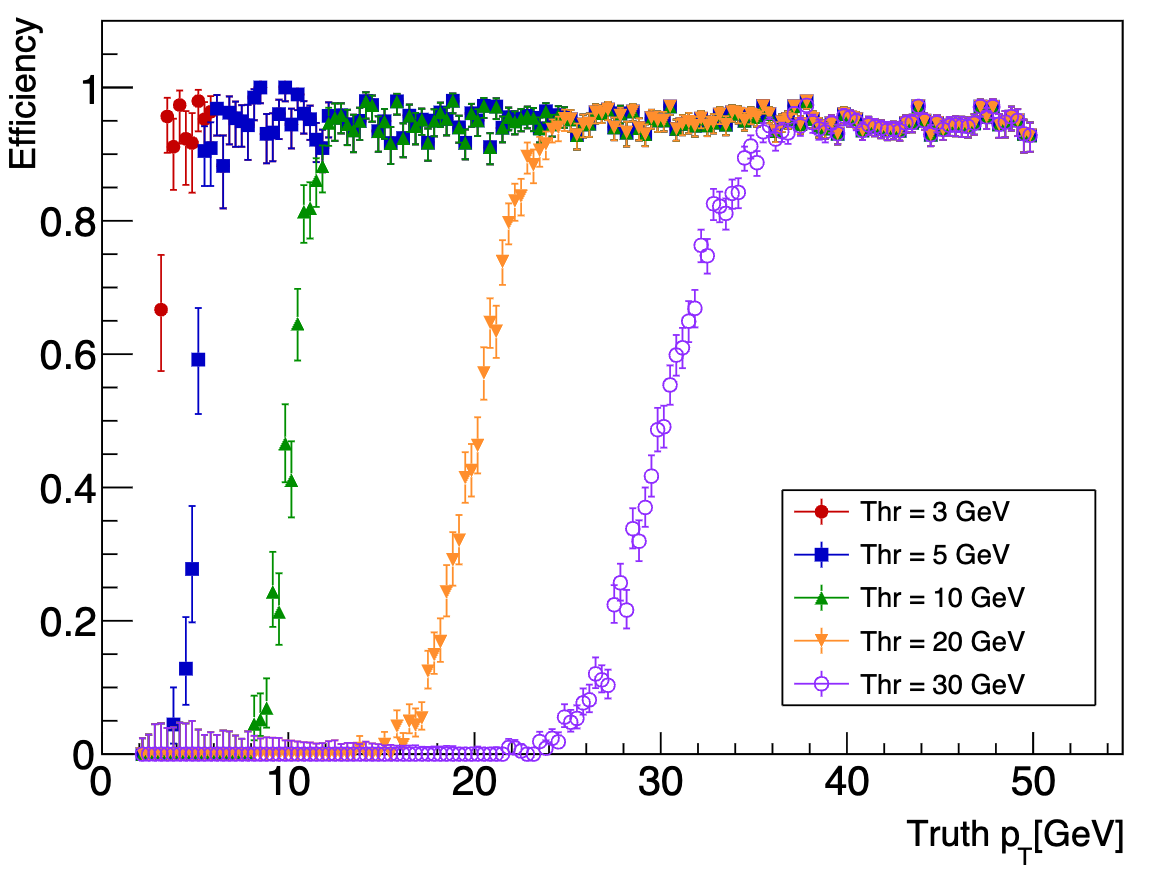
\includegraphics[width=0.83\textwidth]{figs/chapter4/efficiency_barrel_multi_right_new_new.png}
  \caption{Efficiency of L0MuonEmulator in the barrel region for five $p_\mathrm{T}$ thresholds: 3~GeV, 5~GeV, 10~GeV, 20~GeV, 30~GeV.}
  \label{fig:eff_pt_barrel}
\end{figure}

Figure~\ref{fig:eta_phi_comparison} gives the two-dimensional $(\eta, \phi)$ acceptance maps: the reference map from Phase-II trigger studies (top) and the efficiency map generated by L0MuonEmulator (bottom). Dashed blue boxes in the panel below indicate the manually masked regions like Figure~\ref{fig:masking}. Only obvious region around $\eta = 0$ and $|\eta| = 0.7$ are qualitatively reproduced, while other smaller inefficiency regions are not reproduced. As a result, obvious ``holes'' are simulated by the masking scheme, especially those areas around $\eta = 0$.

\begin{figure}[htbp]
  \centering
  \includegraphics[width=0.8\textwidth]{figs/chapter4/Trigger_acceptance_map_3_4_BI_BO.pdf}
  \vspace{0.5em}
  
  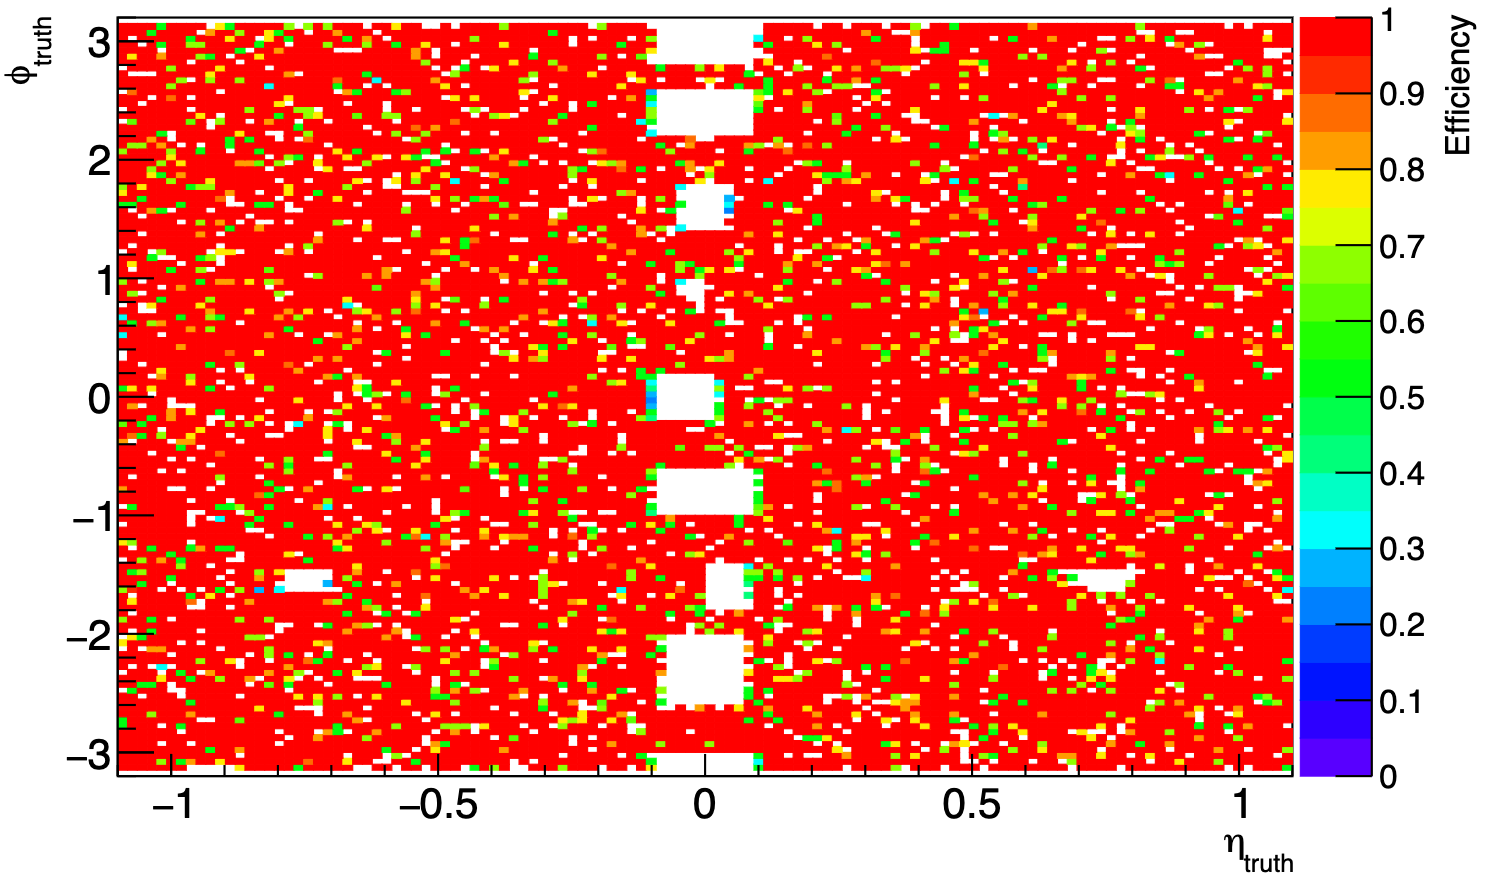
\includegraphics[width=0.83\textwidth]{figs/chapter4/efficiency_eta_phi_2D_new.png}
  
  \caption{Comparison of trigger acceptance maps in the $(\eta, \phi)$ plane of barrel region. Top: Reference acceptance from Phase-II studies. Bottom: Emulator efficiency map including manually masked regions with $p_\mathrm{T}$ threshold of 3~GeV.}
  \label{fig:eta_phi_comparison}
\end{figure}

In conclusion, according to the efficiencies on both $p_\mathrm{T}$ and $(\eta, \phi)$ plane, the behavior of the efficiency is not well reproduced, since it merely parameterize the efficiency, assuming that it is uniform across the angular range except for the holes implemented. Therefore, a complete simulator of high precision that simulates the trigger logic in full detail is still necessary for the Athena implementation. This motivates the implementation of the simulator for TGC Sector Logic, which will be introduced in the next chapter.
